\chapter{Chain Drive Design}
%\section*{Nomenclature}
%\begin{tabular}[t]{p{0.05\linewidth}p{0.4\linewidth}}
%	$ [i] $ & permissible impact times per second\\
%	$ [s] $ & permissible safety factor\\
%	$ [P] $ & permissible power,$ \unit{kW} $\\
%	$ [\sigma_H] $ & permissible contact stress,$ \unit{MPa} $\\
%	$ A $ & cross sectional area of chain hinge,$ \unit{mm^2} $\\
%	$ a $ & real center distance,$ \unit{mm} $\\
%	$ a_i $ & estimated center distance,$ \unit{mm} $\\
%	$ a_{max} $ & maximum center distance,$ \unit{mm} $\\
%	$ a_{min} $ & minimum center distance,$ \unit{mm} $\\
%	$ B $ & width between inner link plate,$ \unit{mm} $\\
%	$ d $ & chordal diameter,$ \unit{mm} $\\
%	$ d_a $ & addendum diameter,$ \unit{mm} $\\
%	$ d_f $ & deddendum diameter,$ \unit{mm} $\\
%	$ d_l $ & roller diameter,$ \unit{mm} $\\
%	$ d_O $ & pin diameter,$ \unit{mm} $\\
%	$ E $ & modulus of elasticity,$ \unit{MPa} $\\
%	$ E_1 $ & modulus of elasticity of the sprockets,$ \unit{MPa} $\\
%	$ E_2 $ & modulus of elasticity of the chain,$ \unit{MPa} $\\
%	$ F_0 $ & sagging force,$ \unit{N} $\\
%	$ F_1 $ & tight side tension force,$ \unit{N} $\\
%	$ F_2 $ & slack side tension force,$ \unit{N} $\\
%	$ F_r $ & force on the shaft,$ \unit{N} $\\
%	$ F_t $ & effective peripheral force,$ \unit{N} $\\
%	$ F_v $ & centrifugal force,$ \unit{N} $\\
%	$ F_{vd} $ & contact force,$ \unit{N} $\\
%	$ i $ & impact times per second\\
%	$ K_d $ & weight distribution factor\\
%	$ k $ & overall factor\\
%	$ \\
%	$ k_{bt} $ & lubrication factor\\
%	$ k_c $ & rating factor\\
%	$ k_d $ & dynamic load factor\\
%	$ \\
%\end{tabular}%
%\begin{tabular}[t]{p{0.05\linewidth}p{0.4\linewidth}}
%	$ k_f $ & loosing factor\\
%	$ k_n $ & coefficient of rotational speed\\
%	$ k_r $ & number of tooth factor\\
%	$ k_x $ & chain weight factor\\
%	$ k_z $ & coefficient of number of teeth\\
%	$ n $ & angular rotational speed, $ arrangement of drive facto\unit{rpm} $\\
%	$ n_{01} $ & experimental angular rotational speed,$ \unit{rpm} $\\
%	$ P_t $ & calculated power,$ \unit{kW} $\\
%	$ p $ & pitch,$ \unit{mm} $\\
%	$ p_{max} $ & permissible sprocket pitch,$ \unit{mm} $\\
%	$ Q $ & permissible load,$ \unit{N} $\\
%	$ q $ & mass per unit length,$ \unit{kg/m} $\\
%	$ s $ & safety factor\\
%	$ v $ & instantaneous velocity along the chain,$ \unit{m/s} $\\
%	$ x $ & chain length in pitches, the number of links\\
%	$ x_c $ & an even number of links\\
%	$ z $ & number of teeth of a sprocket\\
%	$ z_{max} $ & maximum number of teeth of the driven sprocket\\
%	$ \sigma_H $ & contact stress,$ \unit{MPa} $\\
%\end{tabular}

\section{Determination of chain drive pitch}
For power transmission purpose, three modes of failure are considered \cite{mott_vavrek_wang_2018}:
\begin{enumerate}
	\item fatigue of the link plate due to replication of tension in the tight side of the chain.
	\item impact of the rollers as they engage the sprocket teeth.
	\item galling between the pins of each link and the bushing on the pins.
\end{enumerate}
\begin{figure}[ht]
	\centering
	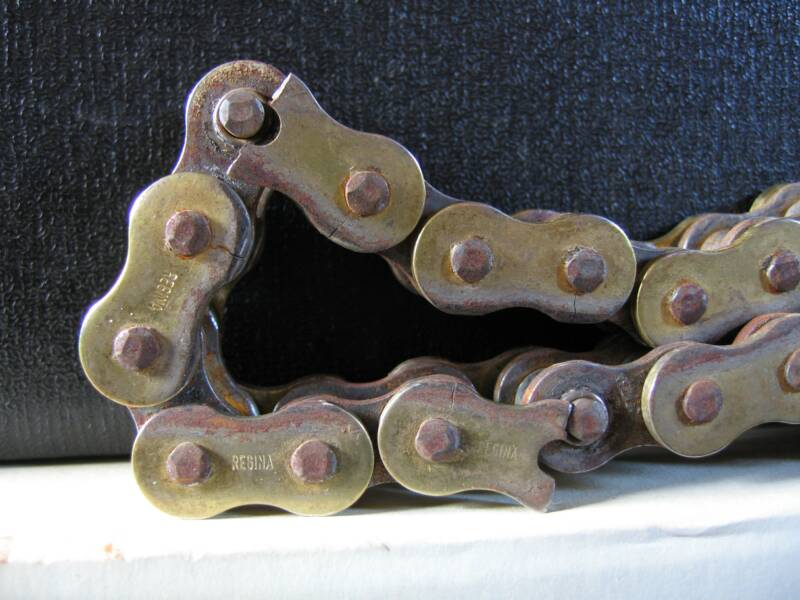
\includegraphics[width=0.5\linewidth]{chain failure}
	\caption{Link plate failure occurs possibly due to overloading}
	\label{fig:chain failure}
\end{figure}

% \textit{Source: sprocketsunlimited.com}

To prevent failure in the chain's service life, one of the methods to find the right pitch is applying strength criterion which is derived into Equation 5.3 \cite{tk1} as permissible power $ [P] $. In this chapter, unless otherwise stated, subscript $ _1 $ is the driving sprocket attached to shaft 3, and $ _2 $ is the driven sprocket attached to the shaft of the mixing tank.

\subsection{Calculate number of teeth of the sprocket $ z $}
The number of teeth $ z $ determines the how stable is the sprocket speed, which relates to the impact intensity and service life. Therefore, $ z_1 $ should be larger than $ 19 $ teeth and $ z_2 $ should be smaller than $ 120 $ teeth, p.80 \cite{tk1}. Similar to gear drives, the wear life in general is improved for hunting tooth ratio \cite{ibt_industrial_solutions}:\\
\[ z_1 = 29 - 2u_{ch} = 29 - 2 \times 2.8 = 25 \geq 19\]
\[ z_2 = u_{ch}z_1 = 2.8 \times 25 = 71 \leq 120\]
where
\begin{itemize}
	\item $ z $ is the number of teeth in a sprocket.
	\item $ u_{ch} $ is given from previous chapter.
\end{itemize}

\subsection{Calculate permissible power $ [P] $ and find pitch $ p $}

An experiment is conducted to find the optimal pitch given the permissible power and angular rotational speed. A roller chain drive having $ 25 $ teeth on the driving sprocket is tested in 8 different cases of $ n_{01} $ in somewhat similar conditions with our design purpose, p.80 \cite{tk1}. In this problem, $ z_1=25 $; $ n_1=n_{sh1}=181.88\unit{rpm} $ is the smaller sprocket speed, which is close to $ n_{01}=200\unit{rpm} $.  $  $ and $   $. The value of calculated power $ P_t $ is:
\begin{multline*}
P_t=P_{ch}kk_zk_n=P_{ch}k_0k_ak_{dc}k_dk_ck_{bt}k_zk_n\\
=6.26\times 1\times 1\times 1\times 1.5\times 1\times 1.3\times 1\times 1.1=10.33\unitp{kW}\leq[P]
\end{multline*}
where
\begin{itemize}
	\item $ k_0 = 1 $ is the arrangement of drive factor, Table 5.6 \cite{tk1}. The centerline between 2 sprockets is parallel with the ground.
	\item $ k_a $ is the center distance factor, Table 5.6 \cite{tk1}. The choice is in the recommended range $ a= (30\div 50)p $, which is similar to the experiment.
	\item $ k_{dc} =1 $ is the chain tension  factor, Table 5.6 \cite{tk1}. The center distance is modifiable through displacing the sprockets.
	\item $ k_d = 1.5 $ dynamic load factor, Table 5.6 \cite{tk1}. The impact load is moderate.
	\item $ k_c = 1 $ is the rating factor, Table 5.6 \cite{tk1}. The system works for 1 shift of 8 hours.
	\item $ k_{bt} =1.3 $ is the lubrication factor, 5.6 \cite{tk1}. Moderate lubrication quality is applied in dusty condition.
	\item $ k_z $ is the teeth ratio, which is used to compare the actual number of teeth with the one in experiment. It is
	\[k_z = {25}/{z_1} = 25/25 = 1\]
	\item $ k_n $ is the speed ratio, which is used to compare the actual speed with the one in experiment. Since $ n_{01}= 200\unit{rpm} $ is closet to $ n_1= 181.88\unit{rpm} $, the ratio is
	\[ k_n = n_{01}/n_1 = 200/181.88= 1.1\]
	\item $ P_{ch} $ is given in Chapter 1.
\end{itemize}
which satisfies the condition.

From $ P_t $ and $ n_{01} $, the permissible power is $ [P] = 11\unit{kW}$, Table 5.5 \cite{tk1}. Also from the table, the pitch is $ p= 25.4 \unit{mm} $, bearing pin diameter $ d_c=7.95\unit{mm} $, inner plate width $ B=22.61\unit{mm} $. Because minimizing damage from impact onto the drive is essential, Table 5.8 \cite{tk1} is consulted. In this case, the pitch is indeed suitable.

\section{Basic parameters of the chain drive}
\subsection{Find $ x_c $}
The recommended value for center distance is in the range $ [a_{min},a_{max}] $, where $ a_{min} = 30p = 30\times 25.4= 762.00 \unitp{mm} $, $ a_{max} = 50p = 50\times 25.4 = 1270.00 \unitp{mm}$ for reducing the effect from chain weight. Since the working area for the system is not given, the lowest value is chosen, $ a = 762.00 \unit{mm} $ to approximate $ x_c $. Then, the value is rounded up to the nearest even number:
\begin{flalign*}
	x_c &= \dfrac{2a}{p} + \dfrac{z_1+z_2}{2} + \dfrac{(z_2-z_1)^2p}{4\pi^2a}\\
	& = \dfrac{2\times 762.00}{25.4} + \dfrac{25+71}{2} + \dfrac{(71-25)^2\times 25.4}{4\pi^2\times 762.00}\\
	& =109.79=112
\end{flalign*}

\subsection{Find center distance $ a $}
Equation 5.13 \cite{tk1} calculates the center distance $ a $ between the sprockets. However, it is also recommended to loose the chain an amount of $ 0.002\div 0.004a $ for tension reduction. Choosing $ 0.003a $ for the averaged value, Equation 5.13 \cite{tk1} is multiplied by an additional amount of $ 0.997 $. Therefore, the center distance is
\begin{flalign*}
	a &= \dfrac{0.997p}{4}\left[x_c-\dfrac{z_2+z_1}{2}+\sqrt{\left(x_c-\dfrac{z_2+z_1}{2}\right)^2-2\left(\dfrac{z_2-z_1}{\pi}\right)^2}\right]\\ 
	&= \dfrac{0.997\times 25.4}{4}\left[112-\dfrac{71+25}{2}+\sqrt{\left(112-\dfrac{71+25}{2}\right)^2-2\left(\dfrac{71-25}{\pi}\right)^2}\right]\\
	&= 788.57 \unitp{mm}
\end{flalign*}
where all the parameters are identified.
%\begin{dmath}
%	a = \dfrac{0.997p}{4}\left[x_c-\dfrac{z_2+z_1}{2}+\sqrt{\left(x_c-\dfrac{z_2+z_1}{2}\right)^2-2\left(\dfrac{z_2-z_1}{\pi}\right)^2}\right] = \dfrac{0.997\times31.75}{4}\left[112-\dfrac{71+25}{2}+\sqrt{\left(112-\dfrac{71+25}{2}\right)^2-2\left(\dfrac{71-25}{\pi}\right)^2}\right] = 788.57 \unitp{mm}
%\end{dmath}

\subsection{Find other parameters} The values below are necessary for modeling the chain drive:\\ 
\[d_1 = p/\sin (180^\circ/z_1) = 25.4/\sin (180^\circ/25) = 202.66\unitp{mm}\]
\[d_2 = p/\sin (180^\circ/z_2) = 25.4/\sin (180^\circ/71) = 574.23\unitp{mm}\]
\[d_{a1} = p \left[ 0.5 + \cot (180^\circ/z_1) \right] = 25.4 \left[ 0.5 + \cot (180^\circ/25) \right] = 213.76 \unitp{mm}\]
\[d_{a2} = p \left[ 0.5 + \cot (180^\circ/z_2) \right] = 25.4 \left[ 0.5 + \cot (180^\circ/71) \right] =  586.37 \unitp{mm}\]
\[d_{f1} = d_1 - 2(0.502 d_l+0.05) = 202.66 - 2(0.502\times 15.88+ 0.05) = 186.60 \unitp{mm}\]
\[d_{f2} = d_2 - 2(0.502 d_l+0.05) = 574.23 - 2(0.502\times 15.88+ 0.05) = 558.17 \unitp{mm}\]
where 
\begin{itemize}
	\item $ d_l=15.88\unit{mm} $ is the roller diameter, Table 5.2 \cite{tk1}.
	\item $ d $ is the chordal diameter,$ \unit{mm} $.
	\item $ d_a $ is the addendum diameter,$ \unit{mm} $.
	\item $ d_f $ is the deddendum diameter,$ \unit{mm} $.
	\item $ p,z_1,z_2 $ are given in previous sections.
\end{itemize}
\section{Strength of chain drive}
\subsection{Impact frequency analysis}
After determining the center distance, it is necessary to validate the impact frequency limit. The condition for impact frequency $ i $ is:
\[i=\dfrac{z_1n_1}{15x_c}=\dfrac{25\times 181.88}{15\times 112}=2.71<[i]=25\]
where
\begin{itemize}
	\item $ [i]=25 $ is the permissible impact frequency, Table 5.9 \cite{tk1}.
	\item $ z_1,n_1,x_c $ are given in previous sections.
\end{itemize}
which satisfies the condition.

\subsection{Safety factor analysis}
Overloading often occurs at the beginning of operation or due to large load, which could damage the chain drive. In order to operate safely, the chain drive's safety factor $ s $ is considered:
\[s = \dfrac{Q}{k_dF_t+F_0+F_v} = \dfrac{56700}{1.2\times 3253.04+120.68+9.63}=19.23 \geq [s] = 7.66\]
where
\begin{itemize}
	\item $ Q = 56700\unit{kN}$ is the permissible load, Table 5.2 \cite{tk1}.
	\item $ k_d=1.2 $ is the dynamic load factor, p.86 \cite{tk1}. The workload is moderate since When turning on the machine, it is around $ 1.5 $ times the amount of the nominal load.
	\item $ F_t $ is the effective peripheral force,$ \unit{N} $. The force is
	\[	F_t = {1000P_{ch}}/{v_1} = {1000\times 6.26}/{1.92} = 3253.04 \unitp{N}\]
	where $ v_1 $ is the instantaneous speed along the chain,$ \unit{m/s} $. The speed is
	\[ v_1={n_1pz_1}/{60000}= {181.88\times 25.4 \times 25}/{60000} = 1.92 \unitp{m/s} \]
	where all parameters are identified.
	\item $ F_v $ is the centrifugal force,$ \unit{N} $. The force is
	\[	F_v =qv_1^2= 2.6\times 1.92^2 = 9.63 \unitp{N}\]
	where $ q=2.6\unit{kg/m} $ is the mass per unit length, Table 5.2 \cite{tk1}.
	\item $ k_d $ is given in previous section.
	\item $ F_0 $ is sagging force,$ \unit{N} $. The force is
	\[	F_0 =9.81\times10^{-3}k_fqa = 9.81\times10^{-3}\times 6\times 2.6\times 788.57 = 120.68\unitp{N}\]
	where
	\begin{itemize}
		\item $ k_f = 6 $ is the sagging factor, Table 5.2 \cite{tk1}. The chain drive is parallel to the ground which is mentioned previously.
		\item $ q,a $ are given in previous sections
	\end{itemize}
	\item $ [s]=7.66 $ is the permissible safety factor, Table 5.10 \cite{tk1}.
\end{itemize}
which satisfies the condition.

\subsection{Contact stress analysis}
For validating contact stress $ \sigma_H $, the following condition must be met, Equation 5.18 \cite{tk1}:
\begin{multline*}
\sigma_H = 0.47\sqrt{\dfrac{k_r(F_t k_d+F_{vd})E}{A K_d}} \\
=0.47\sqrt{\dfrac{0.42\times(3253.04\times 1.5+ 6.22)\times 148975.16}{180\times 1}} = 476.25 \unitp{MPa}\\
\leq [\sigma_H] = 500\unit{MPa}
\end{multline*}
where
\begin{itemize}
	\item $ [\sigma_H] =500\unit{MPa} $ is the permissible contact stress, Table 5.18 \cite{tk1}. From the table, several conditions have to be met. Since $ z_2=71>30 $ and $ v_1=1.92\unit{mm}<5 \unit{mm} $. Thus the suitable material for the sprockets is quenched 45 steel. Another reason supporting the choice  is that a considerable amount of power transmission is shared from the speed reducer.
	\item $ k_r=0.42 $ is the tooth factor. p.87 \cite{tk1}. The value is estimated from $ z_1 $.
	\item $ F_{vd} $ is the contact force,$ \unit{N} $. The force is
	\[ F_{vd} = 13\times10^{-7}n_1 p^3 = 13\times10^{-7} \times  181.88 \times 25.4^3 = 6.22 \unitp{N} \]
	where all the parameters are identified.
	\item $ E $ is the equivalent modulus of elasticity, $ \unit{MPa} $. It is calculated as
	\[E = \dfrac{2E_1E_2}{E_1+E_2} = \dfrac{2\times 205000\times 117000}{205000 + 117000}= 148975.16 \unitp{MPa}\]
	where
	\begin{itemize}
		\item $ E_1 = 205000 \unit{MPa} $ is the modulus of elasticity of the sprockets. The value is found on an online research paper \cite{Mareau2013ExperimentalAN}.
		\item $ E_1 = 117000 \unit{MPa} $ is the modulus of elasticity of the chain, whose material is cast iron ASTM-A48 No. 30A \cite{mott_vavrek_wang_2018}. It is chosen to keep $ \sigma_H $ below $ [\sigma_H] $.
	\end{itemize}
	\item $ A = 180 \unit{mm^2} $ is the cross sectional area of the chain hinge, Table 5.12 \cite{tk1}. The area depends on the pitch value.
	\item $ K_d =1 $ is the number of strands factor. The chain drive only has one strand.
	\item $ F_t, k_d $ are found in previous sections.
\end{itemize}
which satisfies the condition.

\section{Force on shaft}
Apply the following equations, p.87 \cite{tk1}:\\
\[ F_2 = F_0 + F_v = 120.68 + 9.63 = 130.31 \unitp{N}\]
\[ F_1 = F_t + F_2 = 3253.04 + 307.55 = 3383.35 \unitp{N}\]
\[F_r = k_xF_t = 1.15 \times 3253.04 = 3741.00\unitp{N}\]
where
\begin{itemize}
	\item $ k_x = 1.15 $ is the chain weight factor, p.88 \cite{tk1}. The chain drive is parallel to the ground.
	\item $ F_1 $ is the tight side tension,$ \unit{N} $.
	\item $ F_2 $ is the slack side tension,$ \unit{N} $.
	\item $ F_r $ is the force on the shaft,$ \unit{N} $.
	\item $ F_0,F_v,F_t $ are found in previous sections.
\end{itemize}

In summary, we have the following table:

\begin{table}[ht]
	\centering
	\caption{Chain drive final specification}
	\begin{tabular}{lp{0.2\linewidth}p{0.2\linewidth}p{0.2\linewidth}}\toprule
		& Chain drive & Driving sprocket & Driven sprocket \\ \midrule
		Material	&	Cast iron ASTM-A48 No. 30A	&	quenched 45 steel		&	quenched 45 steel		\\
		$ a\unitp{mm}    $	&	788.57	&	-		&	-		\\
		$ B\unitp{mm} $	&	22.61	&	-		&	-		\\
		$ d\unitp{mm} $	&	-		&	202.66	&	574.23	\\
		$ d_a\unitp{mm} $	&	-		&	213.76	&	586.37	\\
		$ d_c\unitp{mm}  $	&	7.95	&	-		&	-		\\
		$ d_f\unitp{mm}  $	&	-		&	186.60	&	558.17	\\
		$ d_l\unitp{mm}  $	&	15.88	&	-		&	-		\\
%		$ i              $	&	2.71	&	-		&	-		\\
%		$ P \unitp{kW}   $	&	11	&	-		&	-		\\
		$ p\unitp{mm}    $	&	25.4	&	-		&	-		\\
%		$ u_{ch}         $	&			&	-		&	-		\\
%		$ v\unitp{m/s}   $	&			&	-		&	-		\\
		$ z              $	&	-		&	25		&	71		\\\bottomrule
	\end{tabular}
\end{table}